\subsection{Разработка архитектуры программного средства}
\label{sec:modeling:sequence_diagram}

В данной архитектуре «Frontend» частью является клиентское приложение. Эта часть системы обменивается данными с серверной, отправляя запросы пользователя в виде HTTP запросов и получая ответы в виде структурированной структуры данных. 

Программное средство создания веб-приложений с помощью готовых графических компонентов является интегрируемым сервисом на стороне клиентского приложения, а не самостоятельным программным средством. Таким образом, разработка общей архитектуры фронтенд части приложения остается за разработчиком, интегрирующим данное программное средство в свой продукт.

Данное программное средство является SPA-приложением, осуществляющим логическую навигацию между своими страницами. Общая схема работы одностраничных приложений показана на рисунке~\ref{sec:design:spa}.
\begin{figure}[ht]
\centering
    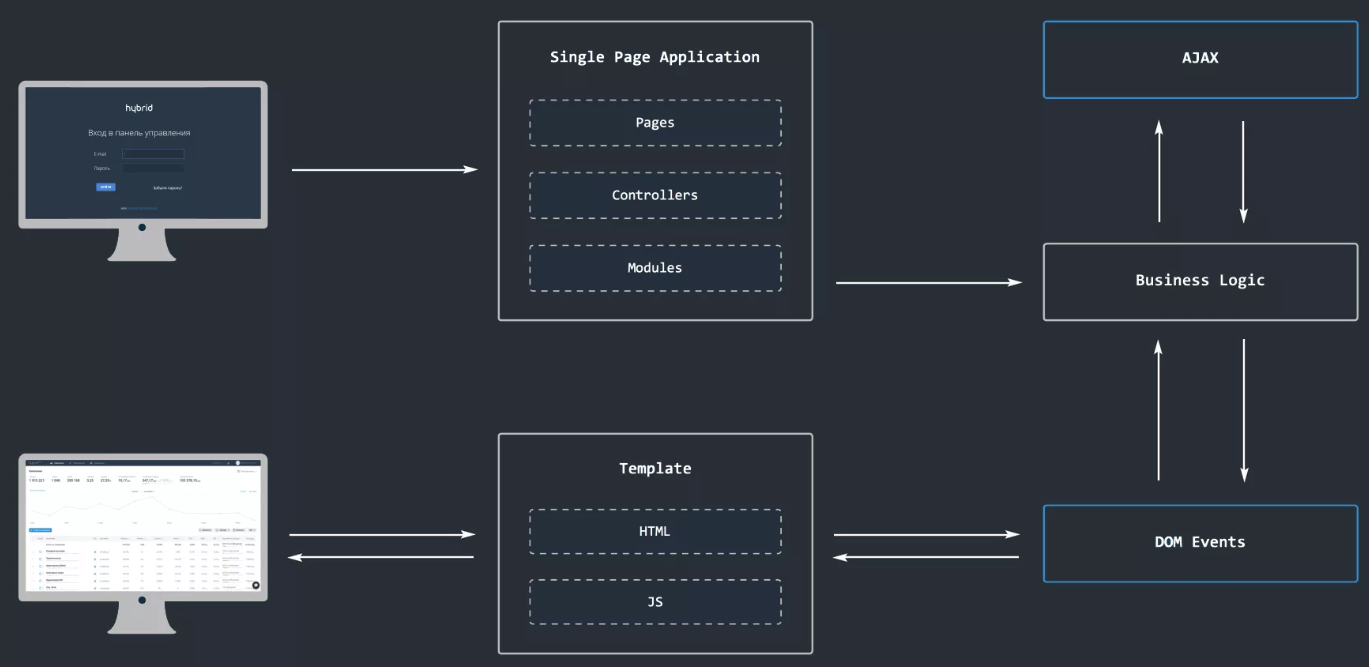
\includegraphics[scale=0.44]{spa.png}
    \caption{Диаграмма последовательности использования предопределенных конфигураций графических компонентов}
    \label{sec:design:spa}
\end{figure}

Программное средство состоит из следующих страниц:

\begin{itemize}
    \item обзорная страница, скрывающая от пользователя <<лишние>> панели, что позволит детальнее осмотреть созданный макет;
    \item страница, содержащая меню, позволяющее пользователю загрузить новые пресеты, предоставляемые разработчиком продукта;
    \item страница компонентов, содержащая основные инструменты и функциональность;
    \item <<песочница>>, предоставляющая пользователю возможность протестировать созданный макет приложения;
    \item страница, содержащая сгенерированный код макета, сохранить макет как пресет.
\end{itemize}

Навигацию между видами осуществляет меню-оболочка. Однако как ее подключение, так и подключение всех перечисленных выше страниц является опциональным и лишь предоставляет дополнительную функциональность, которая в будущем может быть, например, подвержена дополнительной монитезации разработком, интегрирующим данное программное средство в свой продукт.

Основной и обяательной страницей является страница компонентов, содержащая главыне инструменты:

\begin{itemize}
    \item палитра компонентов, осущестляющая загрузку компонентов и пресетов и предоставляющая доступ к их спискам;
    \item инспектор свойств, содержащий меню доступа к свойствам компонентов, настройкам привязки и т.д.;
    \item грид-разметка, несущая основную функциональность, является местом создания макетов.
\end{itemize}

Расположение компонениов никак не влияет на функциональность, так что этот пункт целиком и полностью остается за разработчиком, интегрирующим данное программное средство в свой продукт.

Основное преимущество заключается в том, что количество одновременно доступных пользователю экзепляров не ограничивается функциональностью, однако есть одно обязательноек исполнению правило: один грид (грид-разметка)может связываться с каким угодно количеством палитр компонентов и инспекторов свойств, но каждый инспектор свойств и каждая палитра компонентов может быть <<связана>> лишь с одним гридом.

Предоставляемая гибкость программного средства дает пространство для разнообразия реализации разработку, например разработчик может реализовать коллаборативный сервис, который будет позволять в режиме реального времени нескольким людям <<собирать>> свое приложение.